%
\hsection{Adding Rows to a Table and Executing Views}%
\label{sec:factory:tableAndView}%
\FloatBarrier%
%
\begin{figure}%
\centering%
%
\subfloat[][%
We double-click on the table~\sqlil{demand} in the \inQuotes{Tables} pane.%
\label{fig:factoryLibreOfficeBaseTableAndView1chooseTableDemand}%
]{\tightbox{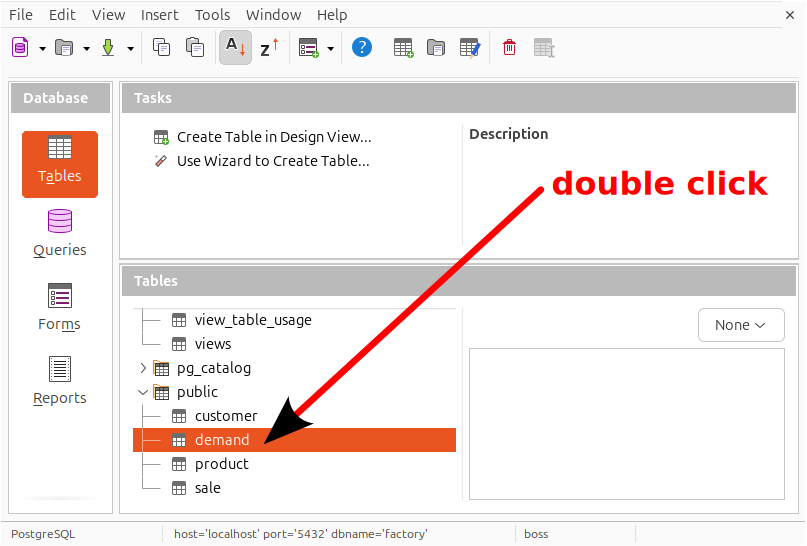
\includegraphics[width=0.49\linewidth]{\currentDir/factoryLibreOfficeBaseTableAndView1chooseTableDemand}}}%
%
\floatSep%
%
\subfloat[][%
The table \sqlil{demand} opens in a separate window, displaying the table content. %
Click into the second cell in the empty row at the bottom.%
\label{fig:factoryLibreOfficeBaseTableAndView2tableDemand}%
]{\tightbox{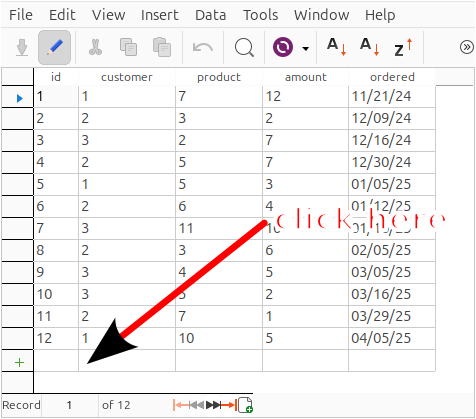
\includegraphics[width=0.49\linewidth]{\currentDir/factoryLibreOfficeBaseTableAndView2tableDemand}}}%
%
\floatRowSep%
%
\subfloat[][%
We enter a new row of data, leaving the \sqlil{id} column empty. %
When reaching the end of row, i.e., after entering all the data, we press~\keys{\tab}.%
\label{fig:factoryLibreOfficeBaseTableAndView3addDemand}%
]{\tightbox{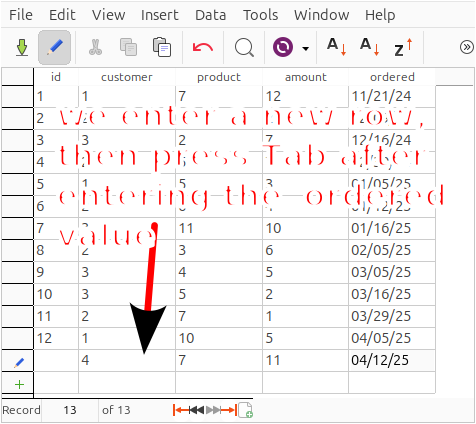
\includegraphics[width=0.49\linewidth]{\currentDir/factoryLibreOfficeBaseTableAndView3addDemand}}}%
%
\floatSep%
%
\subfloat[][%
The row has now been sent to the \dbms. %
It has not been loaded back from the \dbms, so the \sqlil{id} is still~0. %
We click on the \inQuotes{reload} option.%
\label{fig:factoryLibreOfficeBaseTableAndView4demandAdded}%
]{\tightbox{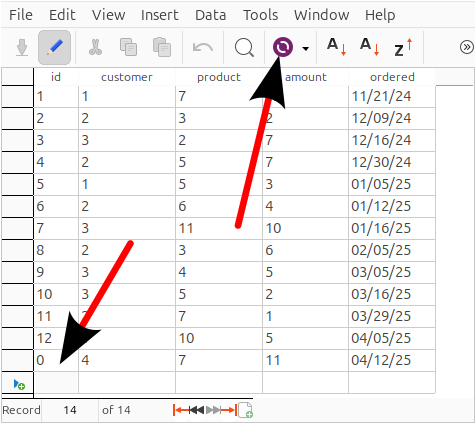
\includegraphics[width=0.49\linewidth]{\currentDir/factoryLibreOfficeBaseTableAndView4demandAdded}}}%
%
\caption{Adding a row to the table \sqlil{demand} and executing the view \sqlil{sale} from \libreofficeBase.}%
\label{fig:factoryLibreOfficeBaseTableAndViewA}%
%
\end{figure}%
%
\begin{figure}%
\ContinuedFloat%
\centering%
%
\subfloat[][%
After refreshing the data by pressing~\libreOfficeBaseRefresh, the \sqlil{id} field is now~13 as it should be.%
\label{fig:factoryLibreOfficeBaseTableAndView5demandsRefreshed}%
]{\tightbox{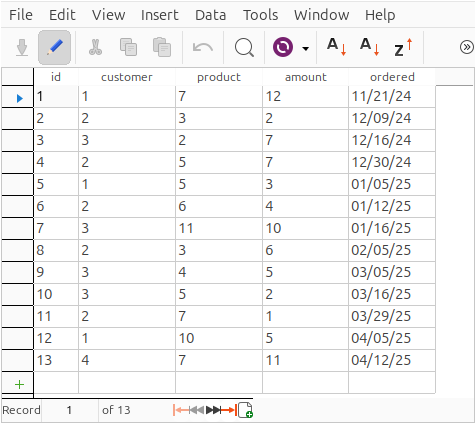
\includegraphics[width=0.49\linewidth]{\currentDir/factoryLibreOfficeBaseTableAndView5demandsRefreshed}}}%
%
\floatRowSep%
%
\subfloat[][%
We now double-click on the view~\sqlil{sale} in the \inQuotes{Tables} pane.%
\label{fig:factoryLibreOfficeBaseTableAndView6chooseViewSale}%
]{\tightbox{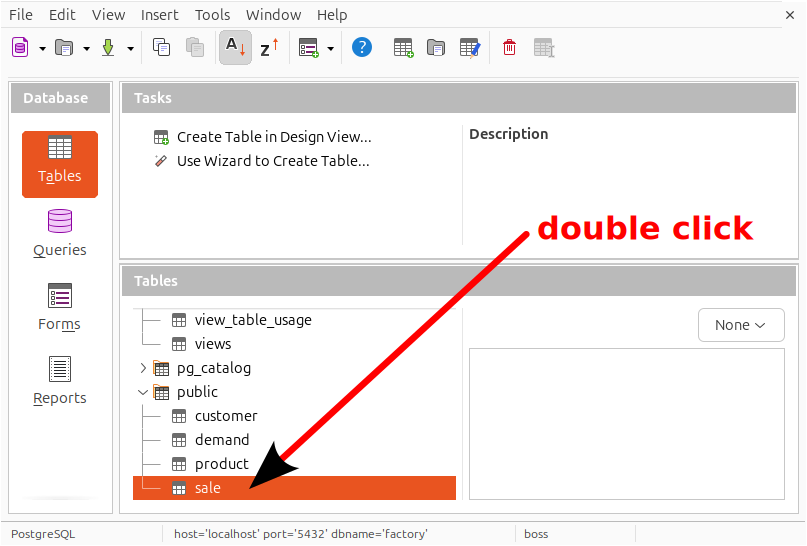
\includegraphics[width=0.49\linewidth]{\currentDir/factoryLibreOfficeBaseTableAndView6chooseViewSale}}}%
%
\floatSep%
%
\subfloat[][%
The view is executed as expected. %
The newly entered demand also showed up: %
There now is a sale for Mr.~Bobbo.%
\label{fig:factoryLibreOfficeBaseTableAndView7viewSale}%
]{\tightbox{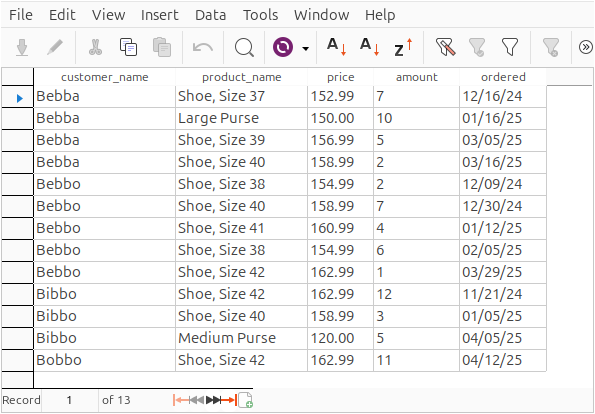
\includegraphics[width=0.49\linewidth]{\currentDir/factoryLibreOfficeBaseTableAndView7viewSale}}}%
%
\caption{Adding a row to the table \sqlil{demand} and executing the view \sqlil{sale} from \libreofficeBase.}%
\label{fig:factoryLibreOfficeBaseTableAndViewB}%
\end{figure}%
%
The first use case of \libreofficeBase\ for our factory \db\ is entering data.
So far, the only method that we know to enter data is via \sql.
This is not suitable for the vast majority of people in an organization.
People are used stuff like \microsoftExcel\ tables or \microsoftWord\ documents.
They are most certainly not be thrilled if they have to learn a programming language for data.
Therefore, we now use \libreofficeBase\ as a simple \pgls{GUI} to enter data into our \db.

We want to use \libreofficeBase\ to interact with a table inside our \postgresql\ \db.
We therefore first open our dokument \textil{factory.odb} using \libreofficeBase.
To connect with the \db, we will have to enter the password \textil{superboss123}.

Now we can select the table \sqlil{demand} in the \inQuotes{Tables}~pane and double-click on it in \cref{fig:factoryLibreOfficeBaseTableAndView1chooseTableDemand}.
A new window opens.
In this window, we see the contents of the table.
The column names are column titles.
Each record is visualized as a row in the table.
This is already good.
As said, many people are used to dealing with the likes of \microsoftExcel\ tables.
This view looks a bit like that.
They can intuitively understand the concept of columns and rows.
This is much clearer and nicer than the output we could get with \psql{\dots}%

We can edit the data right in this view.
We can also add new records.
Therefore, we place the cursor into the second field of the empty row at the bottom~\cref{fig:factoryLibreOfficeBaseTableAndView2tableDemand}.
(We skip the \sqlil{id} column, because its value can automatically be set by the \dbms.)
As data, we choose Mr.~Bobbo and thus enter customer id~4 in~\cref{fig:factoryLibreOfficeBaseTableAndView3addDemand}.
On April~12, 2025, he ordered 11 units of the product with id~7, i.e., shoes of size~37.
After entering this data, when our cursor is in the last cell of the row, we press~\keys{\tab}.

The new record is sent to the \dbms\ in~\cref{fig:factoryLibreOfficeBaseTableAndView4demandAdded}.
Notice that, at this stage, the window displays the \sqlil{id} field of the new row as~0.
The reason is that we did not enter any value here.
The system has sent the new record to the \dbms.
The \dbms\ then sets the \sqlil{id} field automatically.
However, the \libreofficeBase\ \pgls{GUI} does not know this.
In order to see the actual value of the field~\sqlil{id}, we have to reload the data.

We therefore click on the refresh button~\libreOfficeBaseRefresh\ in \cref{fig:factoryLibreOfficeBaseTableAndView5demandsRefreshed}.
Indeed, now the \sqlil{id} field of our new record has the new and correct value~13.
We close the table window and go back to the main window.

A \pgls{db} view provides an application with a perspective on the data.
A view looks a bit like a table but is actually something like a solidified \sql\ query.
We can also access views from \libreofficeBase\ and there, too, they look like tables.

Back to the \inQuotes{Tables} pane we now double-click on the view \sqlil{sale} in \cref{fig:factoryLibreOfficeBaseTableAndView6chooseViewSale}.
This again opens a new window in \cref{fig:factoryLibreOfficeBaseTableAndView7viewSale}.
We now see the results of the query in a nice tabular form.
It may be that the \sqlil{customer_name} column is displayed a bit odd on your computer.
In this case, just resize it and make it a bit wider by dragging its right border to the left with the mouse.
Then all the data will appear correctly.

Remember that above, we just added a new demand into our table?
Back in \cref{exec:factory:select_from_view_sale_3}, there was not a single order for Mr.~Bobbo in our system.
But now a new one appears in the view window, at the bottom row.
In other words, the view has been executed and led to the expected results.
It also confirms that our changes to the \db\ were indeed persistently stored.

At this stage, we can already see an important benefit of using a \pgls{GUI} like \libreofficeBase.
We can now enter and view the data in our tables much more conveniently.
Before, we had to imagine the abstract tabular form of our tables.
But now, we can really see and edit them as actual tables.
This provides much better haptics to our \db.
With an interface like that, a normal user could already work.
That's quite nice.%
%
\FloatBarrier%
\endhsection%
%
